\documentclass[a4paper,10pt]{article}

\usepackage[utf8]{inputenc}
\usepackage[T1]{fontenc}
\usepackage[francais]{babel}
\usepackage{amsmath}
\usepackage[top=3cm, bottom=3cm, left=2cm , right=2cm]{geometry}
\usepackage{graphicx}

\title{\vspace{-2cm}Projet optimisation d'un hélicoptère en papier}
\author{Mines Saint-\'Etienne, Data Science,  2016\:-\:2017 }
\date{}

\begin{document}
\maketitle

\subsection*{Description du problème}

\paragraph{}
L'objectif général du projet est de minimiser la vitesse de chute d'un hélicoptère en papier en utilisant des outils de planification d'expériences et méta-modélisation. Les hélicoptères sont constitués d'une base, de deux ailes et de deux bras de renfort qui, une fois pliés, constituent le rotor d'un hélicoptère (cf. schéma ci-dessous). Deux trombones sont accrochés au bas du corps pour stabiliser l'hélicoptère et attacher les bras.

\begin{center}
	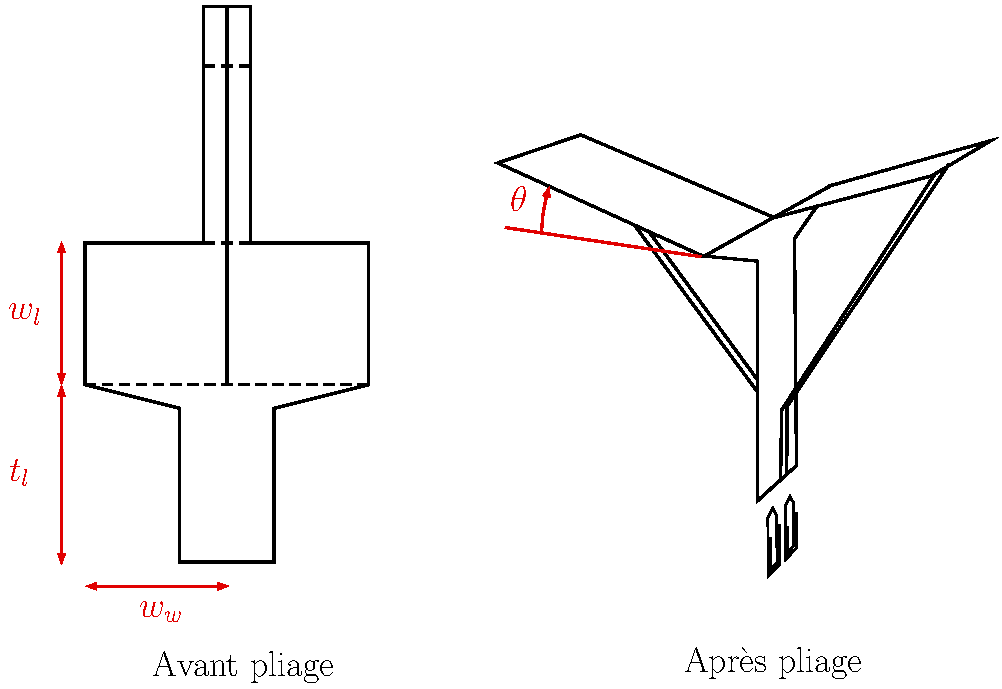
\includegraphics[width=9cm]{figures/newhelico.pdf}
\end{center}

\paragraph{}
Afin de maximiser le temps de vol, on pourra faire varier 4 paramètres: la largeur des pales $w_w$ (\emph{wing width}), la longueur des pales $w_l$ (\emph{wing length}), la longueur de la base $t_l$ (\emph{tail length}), ainsi que l'angle des pales $\theta$. 

\paragraph{}
Le temps de vol d'un hélicoptère, $T$,  peut être considéré comme une variable aléatoire (aléas dus aux courants d'air, à la manière de lâcher, à l'incertitude de mesure, etc.). On réalisera donc plusieurs lâchers depuis le niveau 2 de la cage d'escalier de l'Espace Fauriel (hauteur de la rambarde), jusqu'au sol du niveau 0. 

\paragraph{}
Des contraintes de bornes sont appliquées sur les variables afin que l'hélicoptère puisse être découpé à partir d'une feuille A4. Les contraintes sur les variables sont les suivantes

\begin{equation*}
20  \leq w_w \leq 50 \, , \qquad 30 \leq w_l \leq 75 \, , \qquad 50   \leq t_l \leq 80 \, , \qquad -15  \leq \theta \leq 25 \, .
\end{equation*}

\subsection*{Déroulement}

Le projet se déroulera sur 6 séances de 1h30 :
\begin{center}
\begin{tabular}{l|l|l}
 TP & Date & Objectif \\
 \hline
 1 & 19/12, 8h15 & Construction de plusieurs plans remplissant l'espace. Les plans seront analysés et \\
 & & comparés et chaque groupe sauvegardera son ``meilleur'' plan.\\
 \hline
 2 & 19/12, 10h & Réalisation des expériences \\
 \hline
 3 & 19/12, 13h30 & Construction et validation d'un premier modèle de krigeage\\
 \hline
 4 & 19/12, 15h15 & Analyse du modèle obtenu, raffinage du plan d'expérience dans le domaine d'intérêt\\
  \hline
 5 & 20/12, 8h15 & Analyse dde sensibilité et recherche de l'hélicoptère optimal l'aide de l'algorithme EGO\\
  \hline
 6 & 20/12, 10h & Finalisation du rapport
\end{tabular}
\end{center}

\subsection*{Évaluation}
Vous travaillerez en groupes de 4. Un rapport est à déposer sur Campus, ainsi que les codes R que vous avez utilisés pour répondre à la problématique. La date limite pour le dépôt est \textbf{le mercredi 21 décembre à minuit}. A titre indicatif, la longueur attendue pour le rapport est de l'ordre de 8-10 pages.

\end{document}
